\begin{Exercise}\label{p:continuas06}
  \textbf{\raisebox{.5pt}{\textcircled{\raisebox{-1.2pt} {E}}}} \textit{a}) Una carga de $\SI{-12.0}{\nano\coulomb}$ está distribuida de manera uniforme en un cuarto de círculo de radio $a = \SI{25.0}{\centi\metre}$ que se encuentra en el primer cuadrante, con el centro de curvatura en el origen, como se muestra en la figura \ref{f:continuas06}. Calcular el campo eléctrico en el origen. \textit{b}) Encontrar el campo eléctrico en el centro de la semicircunferencia de radio $R$ y densidad de carga lineal uniforme $\lambda$ mostrada en la figura \ref{f:continuas07}.
\end{Exercise}
\begin{Answer}
  \begin{minipage}[t]{.4\textwidth}
    \textit{a}) $|\va*{E}| = \SI{1556}{\newton/\coulomb}$; $\theta = 45^\circ$\\ \textit{b}) $\va*{E} = \dfrac{\lambda}{2\pi\varepsilon_o R}\vu{x}$
  \end{minipage}
\end{Answer}
%
\begin{center}
  \begin{tikzpicture}[scale=0.6]
    \draw [very thick] (3,0) arc (0:90:3);
    \draw [blue, -{latex}] (0,0)--(2.12,2.12) node[midway, above] {$a$};
    \draw [blue, -{latex}] (0,-2)--(0,4) node[left] {$y$};
    \draw [blue, -{latex}] (-2,0)--(4,0) node[below] {$x$};
  \end{tikzpicture}
  \captionof{figure}{Problema \ref{p:continuas06} (\textit{a})\label{f:continuas06}}
\end{center}
%
\begin{center}
  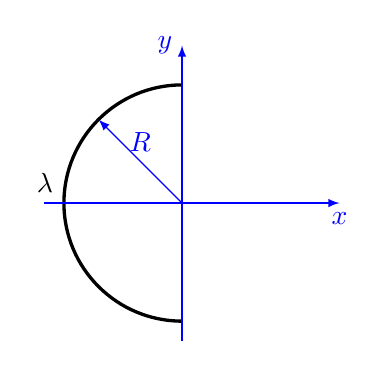
\begin{tikzpicture}[scale=0.5]
    \draw [very thick] (0,3) arc (90:270:3) node[midway, above left] {$\lambda$};
    \draw [blue, -{latex}] (0,0)--(-2.12,2.12) node[midway, above] {$R$};
    \draw [blue, -{latex}] (0,-3.5)--(0,4) node[left] {$y$};
    \draw [blue, -{latex}] (-3.5,0)--(4,0) node[below] {$x$};
  \end{tikzpicture}
  \captionof{figure}{Problema \ref{p:continuas06} (\textit{b})\label{f:continuas07}}
\end{center}
%
